\section{Naive Bayes}
\subsection{Model Implementation}
The Naive Bayes model implemented for predicting customer churn in the Telco dataset is a mixed model designed to handle both categorical and numeric features. The model begins with parameter validation, ensuring proper handling of Laplace smoothing for categorical features and variance smoothing for numeric features. During the fitting process, the dataset is split by class labels to calculate class priors and extract categorical and numeric feature indices. For categorical features, probabilities are calculated using Laplace smoothing, and for numeric features, the model computes class-wise means and variances, adding a small variance boost to prevent numerical instability. In the prediction phase, the model computes likelihoods for categorical features based on precomputed probabilities and applies the Gaussian probability density function for numeric features. To ensure stability, log-likelihoods are used, combining the contributions from both feature types and class priors to make predictions. The implementation integrates key machine learning practices like input validation and model persistence while leveraging the simplicity and efficiency of the Naive Bayes approach for churn prediction.

\subsection{Training Implementation}
The training implementation for the Naive Bayes model follows a structured process to handle both categorical and numeric features effectively. The first step is input validation, ensuring the provided data matches expectations. The model verifies the dimensions of the feature matrix and checks that the categorical feature mask aligns with the number of features. It also calculates the class priors by counting occurrences of each class in the target variable, which helps in determining the baseline probability for each class before considering the feature values.\\

For categorical features, the model computes conditional probabilities using a frequency-based approach with Laplace smoothing to prevent zero probabilities when unseen categories appear in the prediction phase. It creates a nested dictionary structure where each class maps to its respective categorical features and their value counts. For numeric features, the model calculates the mean and variance for each feature per class, ensuring stability by adding a small variance boost proportional to the maximum variance across features. This variance smoothing prevents numerical instability when feature variances are very small. These computations ensure the model captures the underlying data distribution effectively, preparing it to make robust predictions across mixed data types.

\subsection{Model Tuning Implementation}
The model tuning process for the Naive Bayes classifier involves using GridSearchCV to optimize the hyperparameters, ensuring the model achieves the best performance across multiple metrics. In this implementation, the laplace smoothing parameter is the focus of the tuning process, which addresses the issue of zero probabilities for unseen categorical values by adding a constant value to all feature counts. A wide range of values is tested, starting from 0.5 and gradually increasing to 200. This comprehensive range allows the model to explore subtle adjustments as well as more aggressive smoothing, helping to identify the optimal balance between bias and variance. Additionally, a Pipeline is used to streamline the process, ensuring the Naive Bayes model is properly integrated into the tuning workflow and preventing data leakage by ensuring transformations happen inside the cross-validation loop.\\

The grid search is performed using k-fold cross-validation, where the dataset is split into k folds, ensuring the model is trained and validated on different subsets of data to prevent overfitting and assess generalizability. The evaluation is conducted across multiple metrics, including accuracy, F1 macro, precision macro, and recall macro, providing a well-rounded assessment of the model’s performance. The refit parameter is set to optimize for accuracy, meaning the final model will be selected based on the best accuracy score. This approach ensures that the model tuning process is thorough, identifying the laplace smoothing value that leads to the most accurate predictions while balancing other important performance metrics. By combining cross-validation, grid search, and multiple evaluation metrics, the model tuning process aims to create a robust classifier that generalizes well to unseen data.

\subsection{Training Process}
The training process for the Naive Bayes model begins by preparing the data and ensuring that it aligns with the expected input format. The fit method is responsible for learning the parameters required for making predictions. First, the training data is validated to ensure its integrity, and the categorical feature mask is checked to match the number of features in the dataset. This mask is crucial, as it determines which features should be treated as categorical and which should be treated as numeric. The model then identifies the indices of categorical and numeric features, which allows it to handle these two types of data differently. Afterward, the training labels are analyzed to determine the unique classes present in the dataset, and the prior probabilities for each class are calculated by dividing the count of each class by the total number of samples. These priors represent the likelihood of encountering each class in the absence of any other information.\\

For categorical features, the model calculates the probability distribution of each feature value within each class using Laplace smoothing. This technique prevents zero probabilities when certain feature values are absent from the training set for a given class. The smoothing parameter ensures that every feature value has a small probability, even if unseen in the training data. The probabilities are stored in a nested dictionary structure, where each class maps to another dictionary containing feature indices, which in turn map to dictionaries of feature values and their associated probabilities. This structure makes it efficient for the model to retrieve probabilities during the prediction phase. The numeric features are handled differently, assuming a normal (Gaussian) distribution. For each numeric feature, the model computes the mean and variance per class, adding a variance smoothing factor to avoid numerical instabilities caused by very small variances.\\

Finally, once the categorical probabilities and numeric feature statistics have been computed, the model saves these parameters for later use in prediction. The training process ensures that the model has learned a set of class priors, conditional probabilities for categorical features, and Gaussian distributions for numeric features. These learned parameters represent the probability distributions needed to classify new data points accurately. Additionally, the model records the total number of features and marks itself as fitted, ensuring that predictions can only be made after the training process has been completed successfully. By carefully separating the handling of categorical and numeric features, the model captures the distinct statistical properties of each type, leading to a more accurate and reliable Naive Bayes classifier tailored to mixed datasets

\subsection{Manual Training Results and Analysis}
For our Naive Bayes model, we manually selected the Laplace smoothing parameter to be 5, which plays a crucial role in handling zero-frequency problems. In traditional Naive Bayes, if a particular feature value does not appear in the training set for a given class, the model assigns a probability of zero to any instance containing that feature, which can severely affect predictions. Laplace smoothing addresses this by adding a constant value (in this case, 5) to the numerator of the probability calculation for each feature-class combination, ensuring no probability is ever zero. Choosing a higher smoothing value reduces the model’s sensitivity to rare events and prevents overfitting, especially when dealing with categorical data. Setting the smoothing parameter to 5 strikes a balance between ensuring unseen feature values have a reasonable probability and avoiding excessive smoothing that could blur meaningful patterns. This choice reflects careful consideration of the model’s ability to generalize better across unseen data while remaining responsive to the underlying distribution in the training set.

\subsubsection{Evaluation and Cross Validation}

\begin{figure}[hbt!]
    \centering
    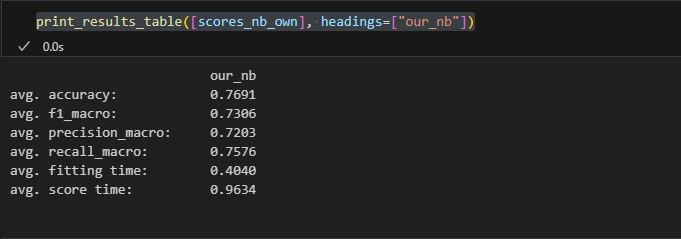
\includegraphics[width=1\linewidth]{Images/6.5a.jpg}
    \caption{Model Evaluation and Cross-Validation Results of Naive Bayes Model}
    \label{fig:enter-label}
\end{figure}

The results of the model training indicate a solid performance with an average accuracy of 0.7691, meaning the model correctly classifies about 76.91\% of instances in the training set on average across cross-validation folds. Accuracy alone doesn’t paint the full picture, so additional metrics offer deeper insights into the model’s effectiveness. The F1 macro score of 0.7306 balances precision and recall across all classes, making it particularly useful when dealing with imbalanced datasets. A macro-averaged F1 score treats each class equally, ensuring that smaller or less frequent classes contribute equally to the overall performance evaluation.\\

Furthermore, the model’s precision macro of 0.7203 suggests that when the model predicts a positive instance for any class, it is correct 72.03\% of the time on average. Precision is crucial in scenarios where minimizing false positives is important. On the other hand, the recall macro of 0.7576 shows that the model correctly identifies about 75.76\% of all true positive instances across classes, indicating its ability to capture most relevant instances without overlooking too many. The training process was also efficient, with an average fitting time of 0.4040 seconds and an average scoring time of 0.9634 seconds. These results highlight the model's robustness with the chosen Laplace smoothing parameter, providing a well-balanced performance in terms of accuracy, precision, recall, and computational efficiency. The combination of these metrics suggests that the model generalizes well across different folds of the dataset, making it a reliable choice for the given task.

\subsubsection{Confusion Matrix}
The confusion matrix shows the performance of the Naive Bayes model with a manually chosen Laplace smoothing parameter of 5. The matrix indicates that the model correctly predicted 2,397 positive instances (True Positives) and 983 negative instances (True Negatives). However, there were 687 instances where the model incorrectly classified negative cases as positive (False Positives) and 152 instances where it failed to detect positive cases, misclassifying them as negative (False Negatives). The model performs well in identifying positive cases, as shown by the high number of True Positives, but the relatively higher number of False Positives suggests that the model leans slightly towards predicting positives. This may be influenced by the chosen smoothing value, which can affect probability estimates and decision boundaries.

\begin{figure}[hbt!]
    \centering
    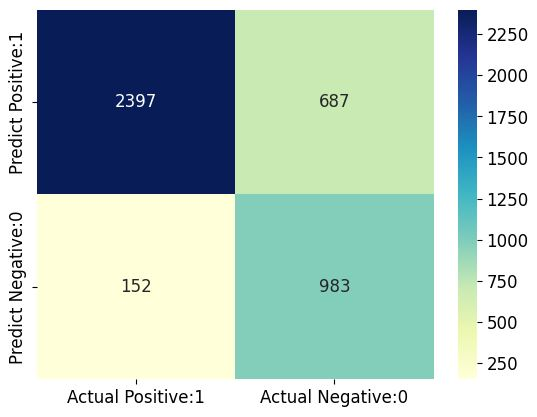
\includegraphics[width=1\linewidth]{Images/6.5b.jpg}
    \caption{Confusion Matrix for Naive Bayes Model}
    \label{fig:enter-label}
\end{figure}

\subsubsection{ROC Curve and AUC Score}

\begin{figure}[hbt!]
    \centering
    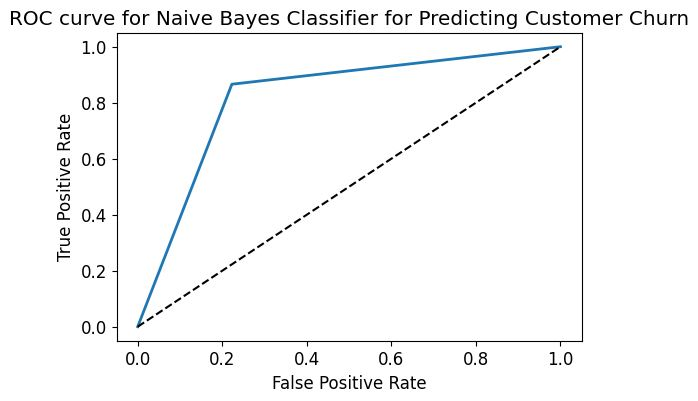
\includegraphics[width=1\linewidth]{Images/6.5c.jpg}
    \caption{ROC Curve for Naive Bayes Model}
    \label{fig:enter-label}
\end{figure}

\begin{figure}[hbt!]
    \centering
    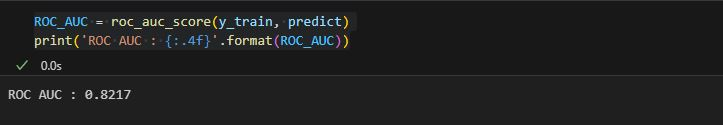
\includegraphics[width=1\linewidth]{Images/6.5d.jpg}
    \caption{AUC Score for Naive Bayes Model}
    \label{fig:enter-label}
\end{figure}

The Area Under the Curve (AUC) score of 0.827 indicates that the Naive Bayes model, with a Laplace smoothing value of 5, demonstrates strong discriminative ability between positive and negative classes. An AUC score ranges from 0 to 1, where 0.5 implies random guessing, and 1.0 represents perfect classification. A score of 0.827 shows that the model can correctly distinguish between classes about 82.7\% of the time, suggesting a well-performing model with good balance between sensitivity and specificity. While the model performs reliably, there is still room for optimization to push the score closer to 1.0, potentially by fine-tuning the smoothing parameter or exploring other feature engineering techniques.

\subsubsection{Precision-Recall Curve}

\begin{figure}[hbt!]
    \centering
    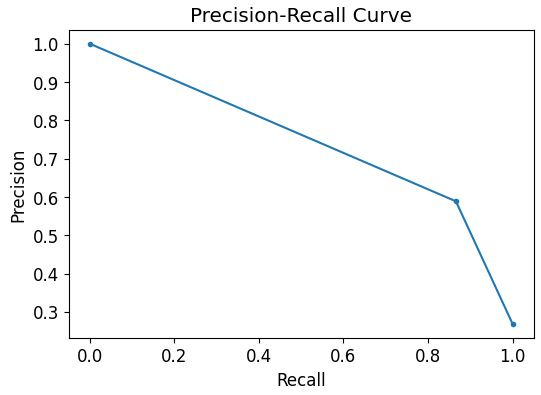
\includegraphics[width=1\linewidth]{Images/6.5e.jpg}
    \caption{Precision-Recall Curve for Naive Bayes Model}
    \label{fig:enter-label}
\end{figure}

The Precision-Recall (PR) curve illustrates the trade-off between precision and recall for the Naive Bayes model with Laplace smoothing set to 5. From the plot, we can see that as recall increases, precision steadily declines. Initially, at very low recall, precision is close to 1.0, indicating that the model makes very few false positives when predicting the positive class. However, as recall rises towards 1.0, precision drops significantly, reflecting that the model captures more true positives at the cost of increasing false positives. This behavior is typical for models where higher recall comes with a trade-off in precision. Analyzing this curve is essential to understanding model performance in imbalanced datasets or scenarios where prioritizing precision or recall impacts the task differently. The gradual slope indicates a relatively stable trade-off, suggesting that the model maintains reasonable precision as recall improves.

\subsection{Model Optimization with Hyperparameter Tuning}
In this model training process, hyperparameter tuning was conducted using GridSearchCV to identify the optimal value for Laplace smoothing in the Naive Bayes model. Laplace smoothing, also known as additive smoothing, addresses the problem of zero probabilities in Naive Bayes classification, which occurs when the model encounters categorical features in the test set that were not present in the training set. Without smoothing, unseen categories result in a probability of zero, which effectively nullifies the entire likelihood for that class. By adding a constant value to each feature count, Laplace smoothing prevents zero probabilities, ensuring the model can still make meaningful predictions for previously unseen feature values. This technique is especially useful in datasets with high cardinality or sparse categorical features, where some combinations of features and classes may not appear during training.\\

\begin{figure}[hbt!]
    \centering
    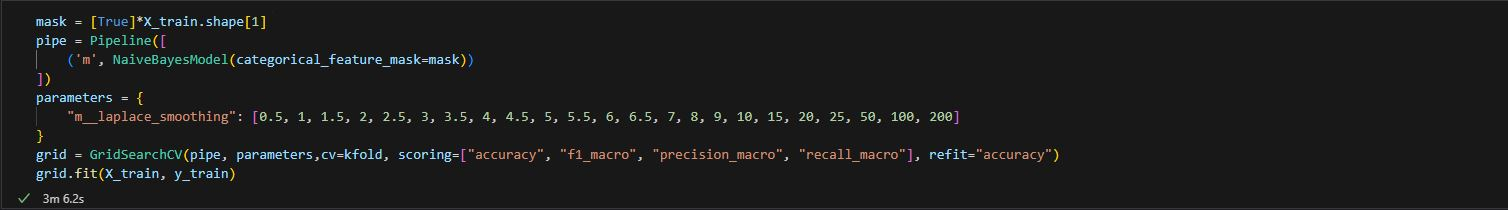
\includegraphics[width=1\linewidth]{Images/6.6b.jpg}
    \caption{Model Tuning using GridSearchCV}
    \label{fig:enter-label}
\end{figure}

In the provided code, a Pipeline was created to streamline the training process by combining data preprocessing and model training into a single workflow. The Naive Bayes model was wrapped in this pipeline with a hyperparameter called laplace smoothing, which determines the amount of smoothing applied. The categorical feature mask was set to True for all features, indicating that every feature in the dataset is treated as categorical. The GridSearchCV function systematically searched through a range of possible values for laplace smoothing — from 0.5 to 200 — ensuring the model explored both low and high smoothing values. This comprehensive search aimed to balance the trade-off between bias and variance in the model's predictions.\\

To ensure robust evaluation, k-fold cross-validation was used, where the training set was split into multiple folds. In each iteration, the model was trained on k-1 folds and validated on the remaining fold, repeating the process k times. This not only prevented the model from memorizing the training data but also provided a more reliable estimate of its performance. The scoring was conducted across multiple metrics like Accuracy, F1-macro, Precision-macro and Recall-macro.\\

The refit="accuracy" argument ensured that after exploring all hyperparameter combinations, the final model would be trained using the hyperparameters that maximized accuracy. This allowed the model to optimize its overall correctness while also providing insights into other performance aspects through the additional scoring metrics.\\

\begin{figure}[hbt!]
    \centering
    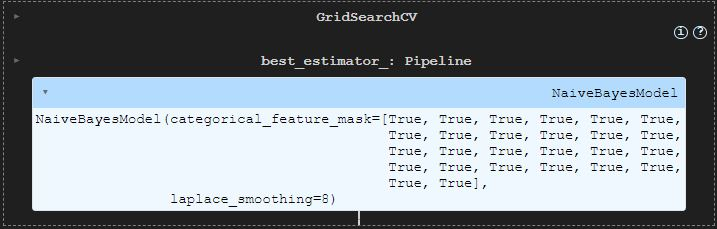
\includegraphics[width=1\linewidth]{Images/6.6a.jpg}
    \caption{Model Tuning Result}
    \label{fig:enter-label}
\end{figure}

After completing the hyperparameter search, the optimal value for Laplace smoothing was found to be 8. This value indicates that adding a smoothing factor of 8 resulted in the best accuracy across the cross-validation folds. The choice of this value suggests a balance between under-smoothing and over-smoothing: If the smoothing value is too low, the model becomes overly confident when encountering unseen categories, as it assigns zero probability to unobserved features, leading to poor generalization. On the other hand, if the smoothing value is too high, the model excessively dilutes the influence of observed data, resulting in overly flat probability distributions and making predictions less sensitive to meaningful patterns in the data.\\

By selecting 8 as the optimal smoothing value, the model effectively mitigated these risks. It applied enough smoothing to handle unseen feature values without overshadowing the contributions of frequently occurring features. This value likely reflects the dataset’s characteristics — possibly a moderate number of categorical features with occasional rare values — making a mid-range smoothing value the best choice. Additionally, the model benefited from a slight bias towards stability by avoiding extreme sensitivity to rare events.\\

The hyperparameter tuning process played a crucial role in enhancing the model’s performance. Through cross-validation, the GridSearchCV procedure ensured that the selected smoothing value generalized well across different data splits, preventing the model from overfitting to specific patterns in the training set. The fact that 8 emerged as the optimal value demonstrates that moderate smoothing worked best for this dataset, ensuring a balance between generalization and predictive accuracy.\\

In summary, the use of GridSearchCV for hyperparameter tuning allowed for a thorough exploration of smoothing values, ultimately enhancing the Naive Bayes model's robustness. The selected smoothing value of 8 suggests that the model benefited from a moderate degree of smoothing, effectively handling unseen features while preserving meaningful patterns in the data. This tuning process not only optimized accuracy but also ensured the model was evaluated across multiple metrics, providing a well-rounded assessment of its performance. The result is a Naive Bayes classifier capable of making stable, reliable predictions even in the presence of previously unseen data points.

\subsection{Optimal Training Results and Analysis}
\subsubsection{Evaluation and Cross Validation}

\begin{figure}[hbt!]
    \centering
    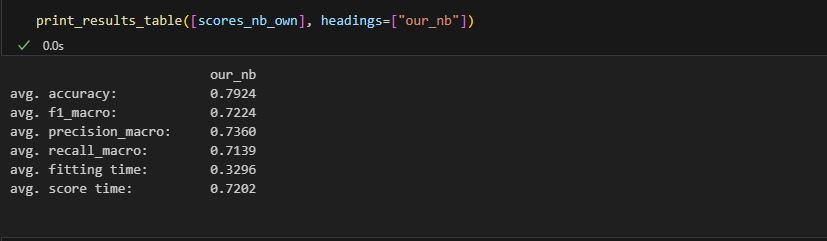
\includegraphics[width=1\linewidth]{Images/6.7a.jpg}
    \caption{Model Evaluation and Cross Validation after Tuning}
    \label{fig:enter-label}
\end{figure}

The results after hyperparameter tuning with Laplace smoothing = 8 show that the Naive Bayes model achieved an average accuracy of 0.7924, meaning the model correctly classified about 79.24\% of the instances across the cross-validation folds. This indicates that the model has learned meaningful patterns from the data and generalizes well to unseen examples. The average f1 macro score of 0.7224 reflects a balance between precision and recall across all classes, which is particularly important in cases of class imbalance, ensuring that both false positives and false negatives are accounted for.\\

The average precision macro of 0.7360 highlights the model's ability to avoid false positives, meaning when the model predicts a class, it is correct about 73.60\% of the time on average across classes. Similarly, the average recall macro of 0.7139 shows the model’s ability to correctly identify positive instances, capturing about 71.39\% of all actual positives across classes. The fitting and scoring times, averaging 0.3296 seconds and 0.7202 seconds respectively, demonstrate that the model is computationally efficient. Overall, these results indicate that the tuned Naive Bayes model effectively balances accuracy and generalization, making it well-suited for handling categorical data with a moderate degree of smoothing. 

\subsubsection{Confusion Matrix}
The confusion matrix after tuning reveals the performance of the Naive Bayes model with Laplace smoothing set to 8. The model correctly predicted 2,513 positive instances (True Positives) and 821 negative instances (True Negatives). However, it also misclassified 571 negative instances as positive (False Positives) and 314 positive instances as negative (False Negatives). This indicates that the model performs well at identifying positive cases, with fewer false negatives, though there are still a notable number of false positives. The balance between true positives and true negatives suggests the model is making reasonably accurate predictions overall, aligning with the earlier reported accuracy and F1 score.

\begin{figure}[hbt!]
    \centering
    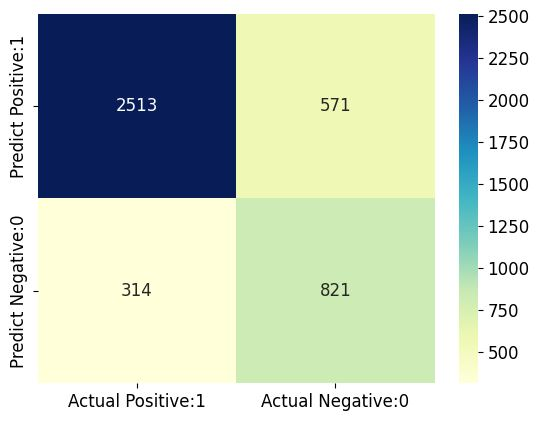
\includegraphics[width=1\linewidth]{Images/6.7b.jpg}
    \caption{Confusion Matrix after Tuning}
    \label{fig:enter-label}
\end{figure}

\subsubsection{ROC Curve and AUC Score}
The ROC curve for the Naive Bayes Classifier after tuning shows a solid balance between true positive and false positive rates, with an AUC score of 0.8325. This indicates that the model has a good ability to distinguish between customers who are likely to churn and those who are not. An AUC of 0.8325 means that if we randomly select one positive instance and one negative instance, there is an 83.25\% chance that the model will correctly rank them. The curve’s rise towards the top-left corner reflects strong performance, suggesting that the tuning process, particularly optimizing the Laplace smoothing parameter, has enhanced the model’s predictive accuracy.

\begin{figure}[hbt!]
    \centering
    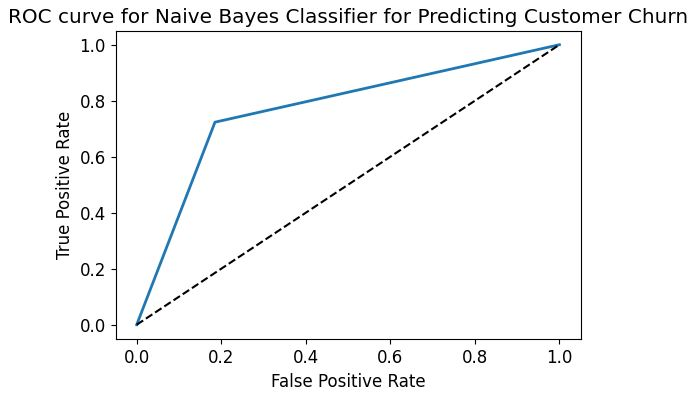
\includegraphics[width=1\linewidth]{Images/6.7c.jpg}
    \caption{ROC Curve after Tuning}
    \label{fig:enter-label}
\end{figure}

\subsubsection{Precision-Recall Curve}
The Precision-Recall (PR) curve after tuning illustrates the trade-off between precision and recall for the Naive Bayes classifier. As recall increases, precision steadily decreases, which is a common pattern in models that aim to balance false positives and false negatives. Initially, when recall is low, precision is very high, meaning the model is confident in its positive predictions. However, as recall increases, the model captures more true positives but at the cost of increased false positives, resulting in lower precision. This behavior reflects the model's capacity to detect churned customers while trying to maintain accuracy in its predictions, showing that tuning has helped in achieving a more balanced performance.

\begin{figure}[hbt!]
    \centering
    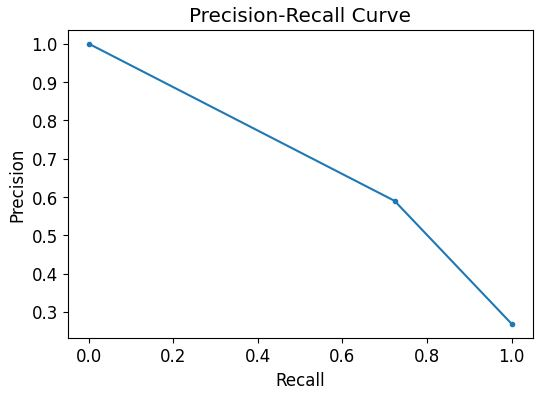
\includegraphics[width=1\linewidth]{Images/6.7d.jpg}
    \caption{Precision-Recall Curve after Tuning}
    \label{fig:enter-label}
\end{figure}

\subsection{Model Comparison}
In this section, we will compare our model after Tuning with two others model that already implemented in the library. The performance comparison between the tuned Naive Bayes model and the two other implementations — Categorical Naive Bayes (CategoricalNB) and Random Forest Classifier — reveals some insightful observations regarding accuracy, macro F1-score, precision, recall, and computational efficiency.\\

\begin{figure}[hbt!]
    \centering
    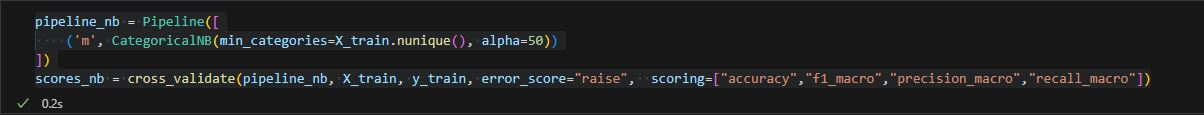
\includegraphics[width=1\linewidth]{Images/6.8a.jpg}
    \caption{CategoricalNB Implementation}
    \label{fig:enter-label}
\end{figure}

\begin{figure}[hbt!]
    \centering
    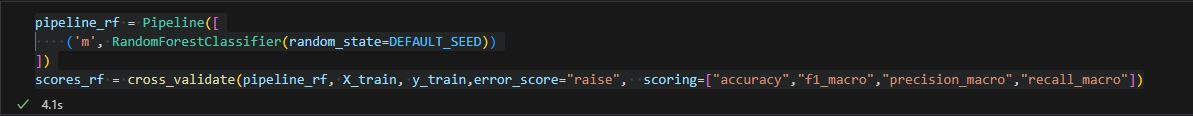
\includegraphics[width=1\linewidth]{Images/6.8b.jpg}
    \caption{Random Forest Classifier Implementation}
    \label{fig:enter-label}
\end{figure}

\begin{figure}[hbt!]
    \centering
    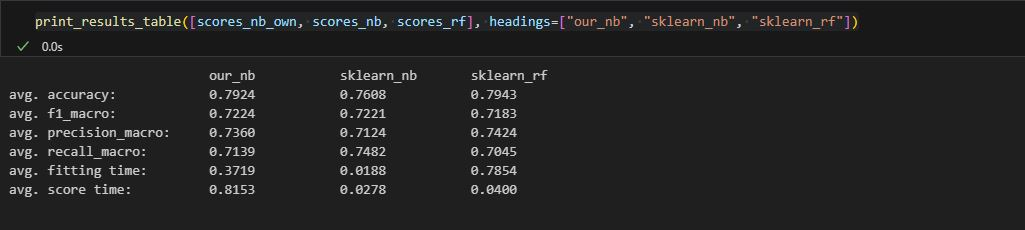
\includegraphics[width=1\linewidth]{Images/6.8c.jpg}
    \caption{Comparison between 3 models}
    \label{fig:enter-label}
\end{figure}

The tuned Naive Bayes model achieves an average accuracy of 0.7924, outperforming both the CategoricalNB model with 0.7608 and the Random Forest Classifier with 0.7943 by a small margin. This indicates that the tuned Naive Bayes model effectively balances correctly predicting both positive and negative cases, making it a strong contender in terms of overall prediction performance.\\

When analyzing the macro F1-score, the tuned Naive Bayes and CategoricalNB show similar results at 0.7224 and 0.7221, respectively, while the Random Forest Classifier falls slightly behind at 0.7183. The F1-score is particularly important for imbalanced datasets as it balances precision and recall, suggesting that the tuned Naive Bayes model effectively handles both false positives and false negatives while maintaining a balanced classification performance across classes.\\

Precision and recall show contrasting strengths between these models. The tuned Naive Bayes has the highest precision at 0.7360, meaning its predictions for the positive class are more reliable compared to CategoricalNB at 0.7124 and Random Forest at 0.7424. In contrast, the CategoricalNB model achieves the highest recall at 0.7482, indicating that it captures more true positives, albeit at the cost of slightly lower precision. The Random Forest Classifier lags behind in recall at 0.7045, suggesting it misses more positive cases than the other two models.\\

Finally, comparing computational efficiency reveals notable differences. The tuned Naive Bayes model's fitting time averages at 0.3719 seconds, significantly longer than the CategoricalNB's 0.0188 seconds but faster than Random Forest's 0.7854 seconds. Similarly, the tuned Naive Bayes model has a longer scoring time of 0.8153 seconds compared to CategoricalNB's 0.0278 and Random Forest's 0.0400 seconds. This indicates that while the tuned Naive Bayes achieves better predictive performance, it comes at the cost of increased computational complexity. Overall, the tuned Naive Bayes model demonstrates the best balance between performance metrics, while the CategoricalNB offers speed and higher recall, and the Random Forest Classifier stands out for precision but with higher computational demands.\\











